\section{Benötigte Trainingsdaten}
Mit wachsender Standortkomplexität werden mehr Trainingsdaten benötigt.
Abbildung \ref{fig:required_training_data} zeigt die benötigten Trainingszyklen für Entscheidungswälder und FFNNs bis auf der Testmenge
eine Klassifizierungsgenauigkeit $P(A)$ von 97\% erreicht wurde.
Es wurde 97\% als Grenze gewählt, da 97,26\% die höchste Klassifizierungsgenauigkeit des FFNNs bei einer Standortkomplexität von 102 ist.
Die Trainingszyklen korrelieren mit der Anzahl der Trainingsdaten, da mit jedem Zyklus die Trainingsdaten ergänzt werden.
\begin{figure}[h!]
    \centering
    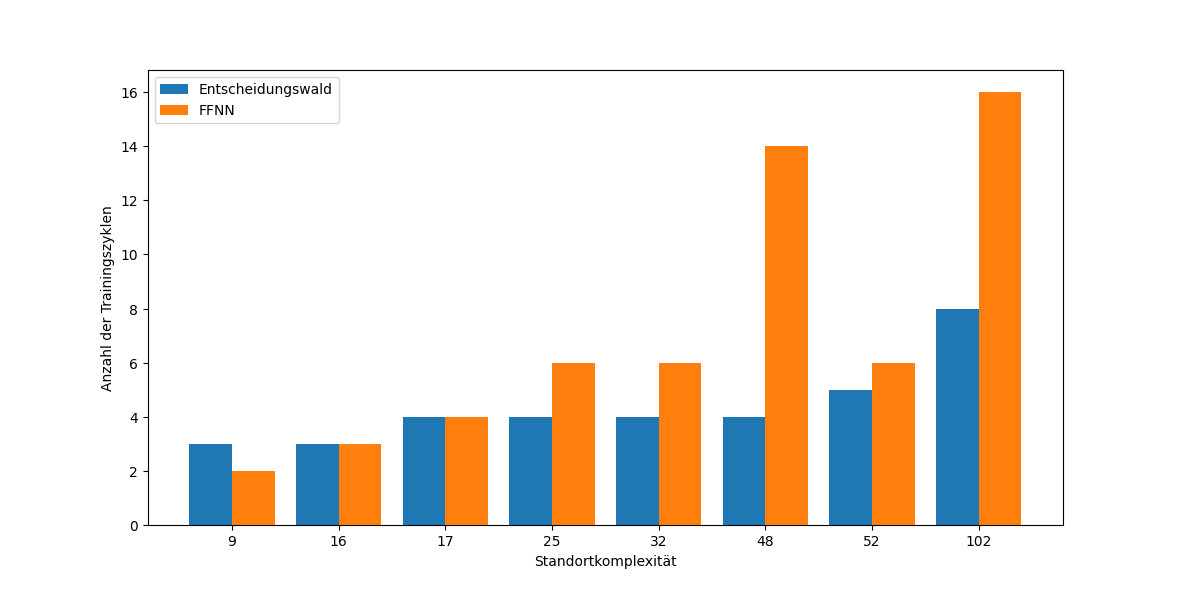
\includegraphics[width=\linewidth]{images/required_training_data.png}
    \caption{Anzahl der benötigten Trainingszyklen bis $P(A)=97\%$ auf der Testmenge erreicht wurde. }
    \label{fig:required_training_data}
\end{figure}
\newpage
Die Entscheidungswälder benötigen weniger Trainingszyklen als FFNNs, um den Schwellenwert zu erreichen.
Je größer die Standortkomplexität, desto größer wird die Differenz der benötigten Trainingsdaten.